\section{Introduction}
\label{sec:introduction}
The Internet offers a vast amount of natural language that can be used in natural language processing, for a very low price. A study by Buck et al.~\cite{buck2014n} estimated that each of the top 10 most frequently used languages on the internet has at least 250 GiB worth of text publically available online. For English (the most frequent), they even found 23 TiB of text.

Such amounts of text have a big potential to be used for the training of language models, but only if building these models can be done in an unsupervised fashion. Manually curating, marking and tagging text is far too much work to be feasible. With unsupervised algorithms, however, the structure in language can be exploited to let computers build language models.

This research will focus on unsupervised training of computer models to translate words. Specifically, we focus on the use of word2vec~\cite{mikolov2013efficient} to provide translations.

\todo{We could expand a bit here, and revisit after writing more of the other parts}

\subsection{Background and Related Work}
\label{sec:prior_work}
Since the introduction of word2vec~\cite{mikolov2013efficient, mikolov2013distributed} in 2013, the algorithm has seen a wide variety of usecases. In the initial paper~\cite{mikolov2013efficient}, Mikolov et. al describe interesting relations between vectors corresponding to words. 
A famous example of how word2vec models relations between words as mathematical equations is $king - man + woman = queen$.
The sematic relationships between man/woman and king/queen are preserved in the transformation of words to vectors, and can be expressed with basic algebra.

Subsequent papers have improved the algorithm both in terms of accuracy (e.g. Levy et al.\cite{levy2014linguistic}), performance, parallelization and extended the initial scope of applications. A good example of the latter is a paper by Boycheva~\cite{boycheva2015distributional}, which uses word2vec outside the natural language processing (NLP) domain but to generate playlists. Based on a set of playlists, their word2vec-based algorithm can suggest new playlists with artists that go well together.

One of the applications of word2vec inside the NLP domain, is exploiting similarities in languages for assistance in machine translation~\cite{wolf2014joint}. Mikolov et al.~\cite{mikolov2013exploiting} released a subsequent paper on word2vec, in which they describe similarities between models of different languages. An example they give, is how the usage of the numbers one to five in English is very similar to the usage in Spanish, and likewise for the names of animals. Figure~\ref{fig:english_spanish} shows a graphical representation of word vectors in English and Spanish.

\begin{figure}[ht!]
  \centering 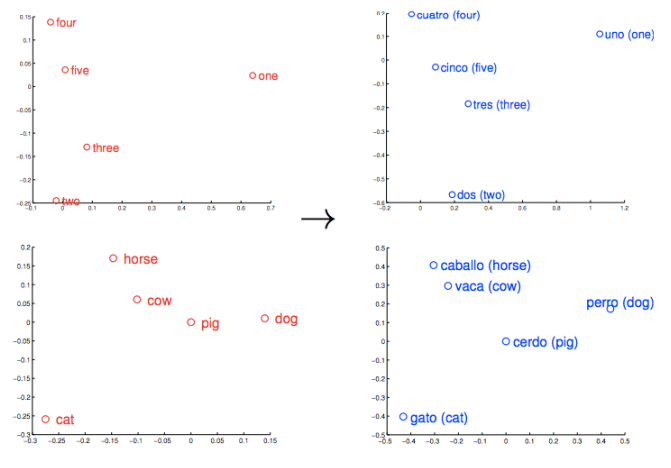
\includegraphics[width=\linewidth]{images/english_spanish}
  \caption{Vector representations of English and Spanish words, after dimensionality reduction and rotation. Notice the high level of similarity between both languages. Reprinted from Mikolov et al.~\cite{mikolov2013exploiting}}
  \label{fig:english_spanish}
\end{figure}

The similarities between languages can be used to predict translations for words without any human interaction or labeled input data. Using only unsupervised machine learning techniques, a computer could learn how to translate English to for instance Spanish and vice versa. The only requirement is a large amount of text in both languages to train the word2vec models on.

In this research, we will focus on this specific application of word2vec: using similarities in languages to provide translations of words.

It is important to note that word2vec only uses information of co-occurrences to model words. It does not learn grammatical concepts other than by statistical analysis. This limits our translation to single words; although the translator might be able to translate each word individually, it cannot learn that each finite verb must has a subject, that "we" is plural, etc. It will learn that "swim" is to "swimming" as "walk" is to "walking", but will not know that "swimming" is a gerund. Note that word2vec can be extended to sentences or whole documents as proposed by Le et al.~\cite{le2014distributed} but this will be out of scope for our research.

\subsection{Our Contribution}
This research aims to improve the capabilities of machines to learn translations with minimal human intervention. Previous research~\cite{mikolov2013exploiting, wolf2014joint} has already shown potential for word2vec in the context of automatic translation, as discussed in section~\ref{sec:prior_work}.

However, we found no practical implementations using Word2Vec and no further research on different setups for word2vec based machine translation.

\subsection{Outline}
We first give a brief summary of word2vec in section~\ref{sec:word2vec}. We then describe three different algorithms for machine translation: one using multiple word2vec models (section~\ref{sec:multi-model-translations}) and two using a single word2vec model (section~\ref{sec:single-model-translations}). In section~\ref{sec:experiments} we describe how the algorithms are tested, and the results of these experiments are in section~\ref{sec:results}. The results are discussed in section~\ref{sec:discussion}.
